\newpage
\chapter{SYSTEM DESIGN}
% \begin{center}
%     \textbf{\LARGE SYSTEM DESIGN}\\[1cm]
% \end{center}

\justify
\section{System Architecture Overview} % (fold)

\begin{figure}[h!]
    \centering
    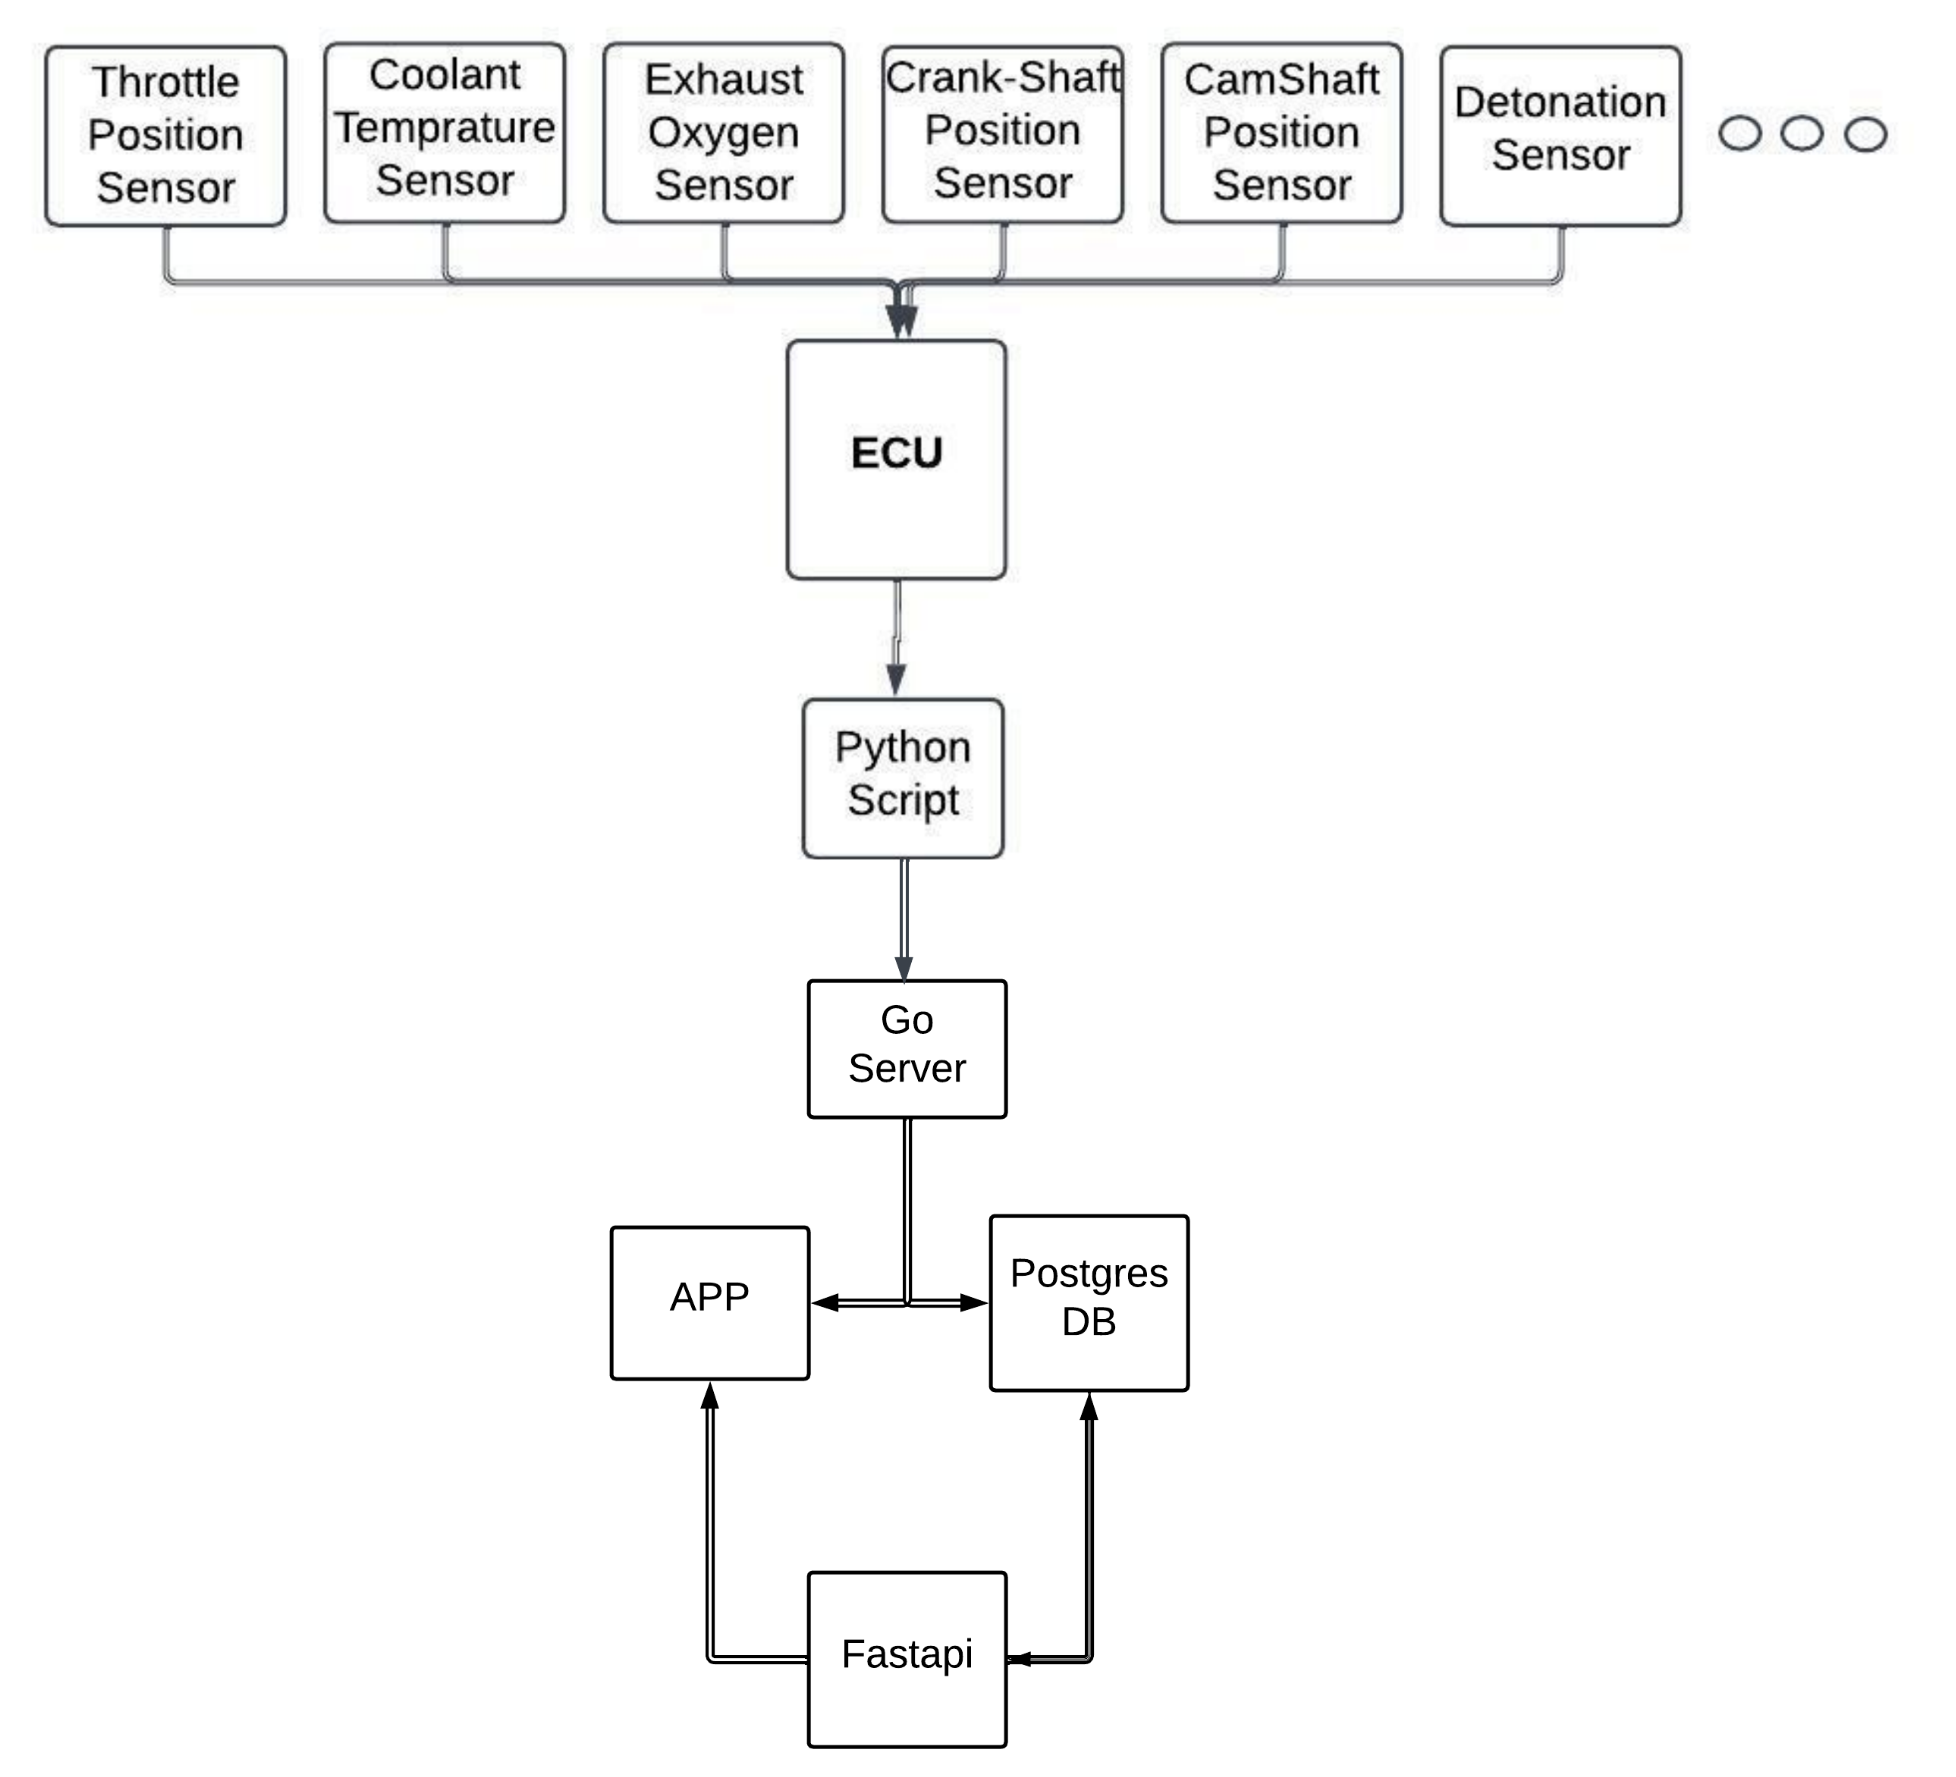
\includegraphics[width=15cm]{assets/system_design_adam.png}
    \caption{System Design Overview}
    \label{fig:system_design_overview}
\end{figure}

The diagram illustrates the flow of data and interactions within an automotive diagnostic and monitoring system. The system integrates multiple sensors, data processing units, databases, and APIs to achieve real-time diagnostics and data sharing. Below is a detailed explanation of the components and their interactions:

\begin{enumerate}
    \item \textbf{Sensors} The system gathers data from a wide range of vehicle sensors to monitor various aspects of vehicle performance and health:
    \begin{itemize}
        \item \textbf{Throttle Position Sensor:} Monitors the position of the throttle to assess acceleration and deceleration patterns.
        \item \textbf{Coolant Temperature Sensor:} Measures the temperature of the engine coolant to monitor engine heat levels.
        \item \textbf{Exhaust Oxygen Sensor (O2 Sensor):} Tracks oxygen levels in the exhaust to evaluate fuel efficiency and combustion quality.
        \item \textbf{Crankshaft Position Sensor:} Detects the rotational speed and position of the crankshaft to ensure proper engine timing.
        \item \textbf{Camshaft Position Sensor:} Monitors the camshaft's rotation to synchronize it with the crankshaft.
        \item \textbf{Detonation Sensor (Knock Sensor):} Identifies engine knock or detonation for optimizing performance and safety.
        \item \textbf{Mass Air Flow (MAF) Sensor:} Measures the mass of air entering the engine to ensure optimal air-fuel mixture.
        \item \textbf{Manifold Absolute Pressure (MAP) Sensor:} Tracks pressure in the intake manifold to monitor engine load.
        \item \textbf{Fuel Pressure Sensor:} Monitors the pressure of fuel in the fuel system to ensure proper delivery to the engine.
        \item \textbf{Oil Pressure Sensor:} Detects oil pressure levels to prevent engine damage due to insufficient lubrication.
        \item \textbf{Transmission Fluid Temperature Sensor:} Monitors the temperature of the transmission fluid to ensure efficient operation.
        \item \textbf{Wheel Speed Sensors:} Measure the rotational speed of each wheel for anti-lock braking and traction control systems.
        \item \textbf{Brake Pedal Position Sensor:} Tracks the position of the brake pedal for braking system diagnostics.
        \item \textbf{Steering Angle Sensor:} Monitors the steering wheel’s position to assess turning angles and stability control.
        \item \textbf{Tire Pressure Monitoring System (TPMS) Sensors:} Measure tire pressure to ensure safety and performance.
        \item \textbf{Ambient Temperature Sensor:} Tracks the temperature outside the vehicle to assist in climate control and engine adjustments.
        \item \textbf{Battery Voltage Sensor:} Monitors the vehicle's battery voltage to detect charging or electrical system issues.
    \end{itemize}
    These sensors send real-time data to the Electronic Control Unit (ECU) for initial processing and control actions.

    \item \textbf{Electronic Control Unit (ECU)} An ECU, or Electronic Control Unit, is the heart and brain of the vehicle, serving as an embedded system in automotive electronics responsible for controlling one or more electrical systems or subsystems in a vehicle. It acts as the central hub that gathers sensor data and error codes, which are accessed via the OBD-II port operating on a client-server architecture. When specific commands are sent to the OBD-II port, it communicates with the ECU and retrieves data in the form of hexadecimal codes. The first two digits of these codes indicate the type of sensor, while the remaining digits represent the corresponding value.\\Modern vehicles often contain numerous ECUs—sometimes over 150—handling various functions such as engine management, transmission control, braking systems, powertrain operations, and more. These ECUs collectively form the vehicle's computer network, enabling diagnostics, advanced functionalities, and seamless control of the vehicle's electrical and mechanical systems.
    \item \textbf{On-Board Diagnostic Port (OBD Port)} On-Board Diagnostics (OBD) is a vehicle's self-diagnostic and reporting capability that monitors the performance of various vehicle subsystems, primarily focusing on emissions control. This system became a requirement in the United States to comply with federal emissions standards, enabling the detection of failures that could lead to excessive tailpipe emissions. The OBD system provides vehicle owners and technicians with access to diagnostic trouble codes (DTCs), which facilitate the identification of malfunctions within the vehicle.\\[1cm]
    
    % image
    \begin{figure}[h!]
        \centering
        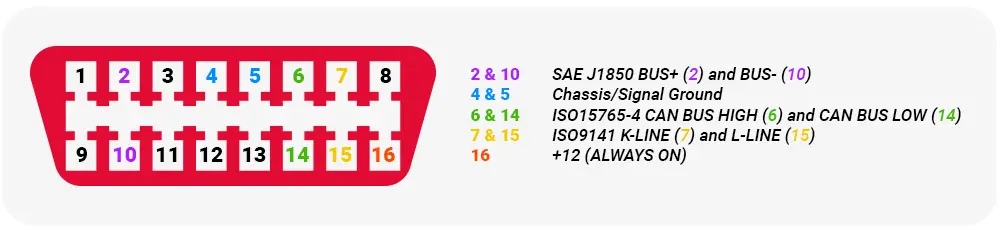
\includegraphics[width=13cm]{assets/obd_pinout.png}
        \caption{OBD-II Connector Pin-out}
        \label{fig:obd_pinout}
    \end{figure}

    The OBD-II standard specifies a 16-pin connector known as the J1962 connector, which is used universally across most vehicles. The pinout for this connector is defined as follows:

\begin{table}[h!]
    \centering
    \caption{OBD-II Connector Pinout}
    \label{table:obd_pinout}
    \renewcommand{\arraystretch}{2.5} % Adjust row height (1 cm approx. with default font size)
    \begin{tabular}{|c|l|}
    \hline
    \textbf{Pin} & \textbf{Function} \\ \hline
    1  & Manufacturer discretion \\ \hline
    2  & Bus positive Line (SAE J1850 PWM and VPW) \\ \hline
    3  & Manufacturer discretion \\ \hline
    4  & Chassis ground \\ \hline
    5  & Signal ground \\ \hline
    6  & CAN high (ISO 15765-4 and SAE J2284) \\ \hline
    7  & K-line (ISO 9141-2 and ISO 14230-4) \\ \hline
    8  & Manufacturer discretion \\ \hline
    9  & Manufacturer discretion \\ \hline
    10 & Bus negative Line (SAE J1850 PWM only) \\ \hline
    11 & Manufacturer discretion \\ \hline
    12 & Manufacturer discretion \\ \hline
    13 & Manufacturer discretion \\ \hline
    14 & CAN low (ISO 15765-4 and SAE J2284) \\ \hline
    15 & L-line (ISO 9141-2 and ISO 14230-4) \\ \hline
    16 & Battery voltage (+12 Volt for type A connector, +24 Volt for type B connector) \\ \hline
    \end{tabular}
    \end{table}
    




The assignment of unspecified pins is left to the vehicle manufacturer's discretion, allowing for variations in implementation across different brands and models.

The communication between the OBD system and the Engine Control Unit (ECU) occurs through standardized protocols. This communication involves several key components:

Data Link Connector: The OBD-II connector serves as a physical interface for diagnostic tools to communicate with the ECU.
Protocols: Various communication protocols are utilized, including:


\begin{itemize}
    \item ISO 9141-2
    \item ISO 14230-4 (Keyword Protocol 2000)
    \item ISO 15765-4 (CAN bus)
\end{itemize}

Parameter Identification (PID): PIDs are specific data points that can be queried from the ECU. They provide information about various vehicle parameters such as engine RPM, vehicle speed, coolant temperature, etc. Each PID corresponds to a specific function or piece of data that the ECU can report back to diagnostic tools.

\item \textbf{Python Script} A Python script retrieves data from the ECU and processes it for further analysis or storage. It acts as a bridge between the raw sensor data and the database/server layer.

\item \textbf{Postgres Database} The Postgres database serves as the primary storage for processed telemetry data. It provides a structured and reliable backend for managing sensor data and results from further computations.

\item \textbf{Go Server} The Go server processes data stored in the Postgres database and performs additional tasks, such as:
\begin{itemize}
    \item Data aggregation
    \item Complex computations or analytics
    \item API responses for connected systems
\end{itemize}
\item \textbf{FastAPI Script} The FastAPI script interacts with the Postgres database to:
\begin{itemize}
    \item Expose APIs for retrieving or upserting data
    \item Enable data queries from other applications or systems
    \item Provide endpoints for monitoring, diagnostics, and reporting
\end{itemize}
\newpage
\item \textbf{Mobile App} The app provides the user interface for interacting with the system. Through the integration with a Golang server and PostgreSQL database, the app can:
\begin{itemize}
    \item Display real-time telemetry data
    \item Provide diagnostic reports
    \item Enable user interaction and configuration of the system
\end{itemize}
\end{enumerate}
